% !TeX spellcheck = de_CH_frami
\section{Ziele}
 \subsection{Use Cases}
 \frame{\frametitle{Use Cases}
 \begin{itemize}
 \item Partner finden
 \item Termin finden
 \item Scores notieren
 \item Regelm�ssige Spiele vereinbaren
 \item Ligen erstellen um regelm�ssige Spiele gegen verschiedene Partner zu vereinbaren 
 \end{itemize}
}
\subsection{Programm}
\frame{\frametitle{Web Applikation und Android Applikation}

\begin{itemize}
\item Ligen erstellen und l�schen
\item Einer Liga beitreten und eine Liga verlassen
\item Spiele vereinbaren
\item Termin f�r Spiel finden
\item Spielresultat eintragen
\item Rangliste der Liga berechnen
\item Automatische Spielvorschl�ge innerhalb einer Liga
\end{itemize}


}



\frame{\frametitle{Schnittstellen}
\begin{itemize}
\item HTTP API f�r alle Funktionalit�ten anbieten
\item HTTP API f�r Android Applikation Benutzen

\end{itemize}
\begin{center}
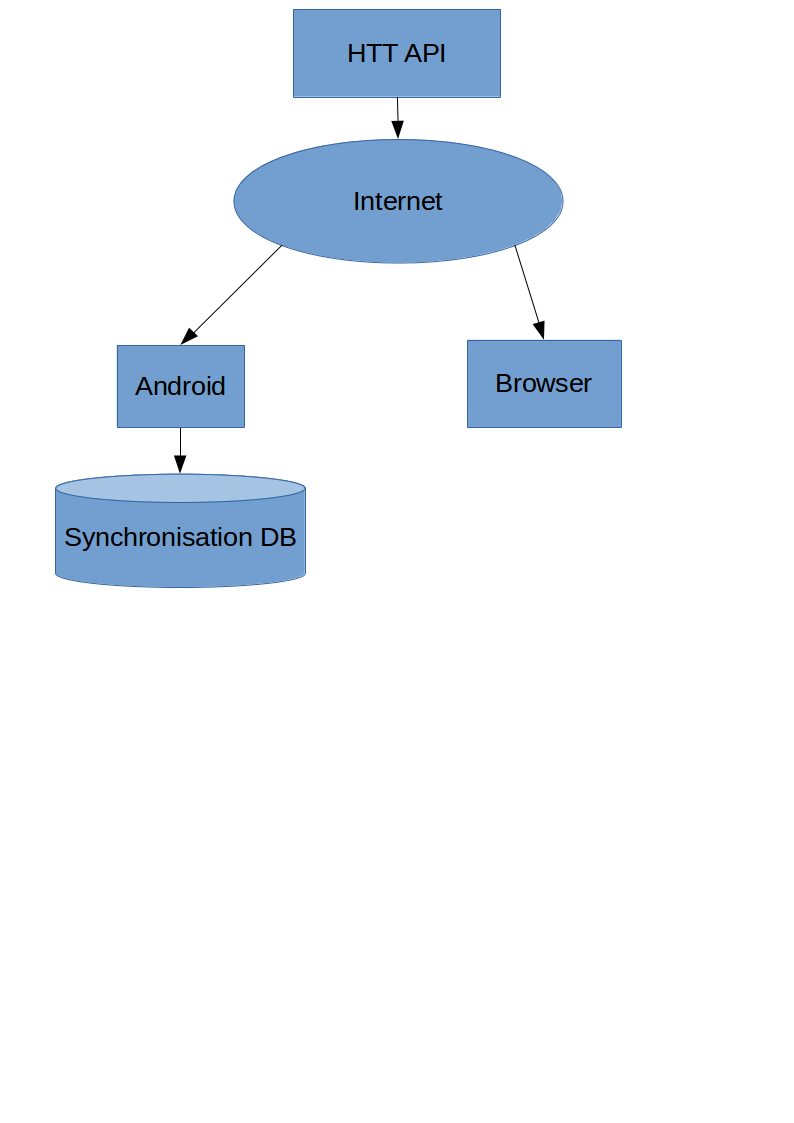
\includegraphics[scale=0.35]{pic/api.png}
\end{center}
}
\frame{\frametitle{Ausblick}
\begin{itemize}
\item Partner finden nach Lokalit�tsprinzip
\item Spontane \glqq Ich will Spielen\grqq{}  Broadcasts zu nahen Spielern
\item Direktbuchung von Courts �ber die Applikation (Monetarisierung)
\end{itemize}
}